\chapter{Fórmula de Euler: forma exponencial de los números complejos}
\chaptermark{Fórmula de \emph{Euler}}

\begin{tikzpicture}
	\fill [left color=red!50, right color=teal!50] (0,0) rectangle (6.5,.2);
	\fill [left color=teal!50, right color=blue!50] (6.5,0) rectangle (11.5,.2);
	\end{tikzpicture}


%\vspace{.5cm}
\section{Repaso de conceptos previos}

\begin{tikzpicture}
	\fill [left color=red!50, right color=teal!50] (0,0) rectangle (3.5,.1);
	\fill [left color=teal!50, right color=blue!50] (3.5,0) rectangle (7.5,.1);
	\end{tikzpicture}
%\vspace{0.5cm}


$z^2+1=0 \ \to \ z=\pm i\, ; \quad i=\sqrt{-1}  \qquad \Rightarrow \qquad z^2-4z+5=0 \ \to \ z=2\pm 2i$


$i^{4n}=1;\quad i^{4n+1}=i;\quad i^{4n+2}=-1;\quad i^{4n+3}=-i$


\begin{multicols}{2}
$z=a+bi\quad $ Forma binómica

$z=r_\theta\quad$ Forma polar

$z=r(\cos \theta+i \sin \theta)\quad $ Forma trigonométrica.

$\begin{cases}
\ \ x=r \cos \theta &|| \quad  r=|z|=\sqrt{x^2+y^2} \\
\ \ y=r \sin \theta &|| \quad  \theta = \arctan y/x 
\end{cases}$

Veremos: $\ \boxed{ \ \subrayado{ \boldsymbol{ z=r\, e^{i\theta} } } \ } \quad $ Forma exponencial
\begin{figure}[H]
	\centering
	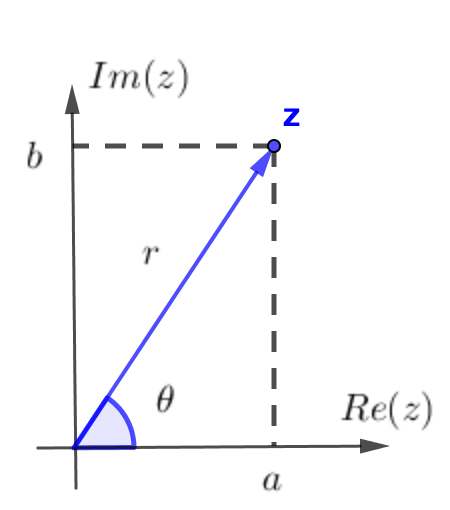
\includegraphics[width=.3\textwidth]{img-complejos/img-comp01.png}
	\end{figure}	
\end{multicols}

Complejo conjugado: Dado $z=a+bi \ \to \  \overline z=a-bi\qquad \qquad  (z\, \overline z=x^2+y^2=r^2)$

En forma binómica, $\quad z_1+z_2=(x_1+iy_1)+(x_2+iy_2)=(x_1+x_2)+i\,(y_1+y_2)\, , \ $

$z_z\cdot z_2=(x_1+iy_1)\cdot(x_2+iy_2)=(x_1x_2-y_1y_2)+(x_1y_2+x_2y_1)\, i \quad \rightarrow  \ (\mathbb C,+,\cdot) \ $ tiene estructura de cuerpo conmutativo.\footnote{Ver Capítulo 1, \emph{`Estructuras algebraicas'} del libro \emph{``Álgebra lineal y geometría (avanzadas) para bachillerato''} de \textsf{Ignacio Vallés Oriola} \\ \textcolor{NavyBlue}{https://github.com/igvaori/algebra-geometria/blob/master/ALGEBRA-LINEAL-Y-GEOMETRIA-A5.pdf}}

División (en forma binómica):$\quad \dfrac {z_1} {z_2} = \dfrac{z_1\, \overline z_2}{z_2 \, \overline z_2}\dfrac{x_1x_2+y_1y_2}{x_2^2+y_2^2}+i\, \dfrac{x_2y_1-x_1y_2}{x_2^2+y_2^2}$

La división, y el producto, son más sencillos en forma polar: 

$\dfrac{z_1}{z_2}=\dfrac{{r_1}_{\theta_1}}{{r_2}_{\theta_2}}= \left( \dfrac{r_1}{r_2} \right)_{\theta_1-\theta_2};\qquad z_1\cdot z_2={r_1}_{\theta_1}\,{r_2}_{\theta_2}=(r_1\, r_2)_{\theta_1+\theta_2}$

Potenciación y radicación: $\quad (r_\theta)^n={r^n}_{n\theta}\, ;\qquad  \sqrt[n]{r_\theta}=\left(\sqrt[n]{r} \right)_{ \frac{\theta+2k\pi}{n} } \, , \ \ n=0,1,2,\cdots k-1$

\textcolor{gris}{Demostración:$\quad \sqrt[n]{r_\theta}=R_\Theta \ \to \ r_\theta=\left( R_{\Theta} \right)^n ={R^n}_{n\Theta}\ \to \ \begin{cases} \ r=R^n & \to R=\sqrt[n]{r} \\ \ \theta=n\Theta & \to  \Theta= \frac{\theta+2k\pi}{n} \end{cases} \quad \Box$}


\vspace{1cm}
\section{La fórmula de \emph{Euler}}

\begin{tikzpicture}
	\fill [left color=red!50, right color=teal!50] (0,0) rectangle (3.5,.1);
	\fill [left color=teal!50, right color=blue!50] (3.5,0) rectangle (7.5,.1);
	\end{tikzpicture}
\vspace{0.5cm}

Recordando los desarrollos de Taylor de la función exponencial, seno y coseno (ver capítulo \ref{DSTaylor}, Desarrollos en serie de Taylor):

$e^x=\displaystyle \sum_{n=0}^{\infty} \dfrac{x^n}{n!}\, ; \qquad \cos \theta= \sum_{n=0}^{\infty} (-1)^n \, \dfrac{\theta^{2n}}{(2n)!}\, ; \qquad \sin \theta= \sum_{n=0}^{\infty} (-1)^n \, \dfrac{\theta^{2n+1}}{(2n+1)!}$

queremos demostrar:


\begin{theorem}

\begin{large}
$$\boxed{ \ \boldsymbol{ e^{i\theta} \ = \ \cos \theta \, + \, i \, \sin \theta
} \ }	\qquad \text{Fórmula de Euler}$$
\end{large}
\end{theorem}

Como $\ i^2=-1 \ \to \ (-1)^n\ $ se puede escribir como: $\ (-1)^n=(i^2)^n=i^{2n}\, , \  $  y además, $\ i(-1)^2=i\, (i^2)^n = i^{2n+1}$

Consideremos un numero complejo de módulo unidad: $1_\theta=\cos \theta + i \sin \theta$:


$\boldsymbol{\cos \theta + i \sin \theta}\  = \ \displaystyle \sum_{n=0}^{\infty} (-1)^n \dfrac{\theta^{2n}}{(2n)!}\, + \, i\, \sum_{n=0}^{\infty} (-1)^n \, \dfrac{\theta^{2n+1}}{(2n+1)!} \ =$

$\displaystyle =  \sum_{n=0}^{\infty} (i)^{2n} \dfrac{\theta^{2n}}{(2n)!}\, + \, i\, \sum_{n=0}^{\infty} (i)^{2n} \, \dfrac{\theta^{2n+1}}{(2n+1)!} \ = \ 
\sum_{n=0}^{\infty}  \dfrac{(i\theta)^{2n}}{(2n)!}\, + \, \sum_{n=0}^{\infty}  \dfrac{(i\theta)^{2n+1}}{(2n+1)!} \ = \ \sum_{n=0}^{\infty} \dfrac{i\theta}{n!}\ = \ \boldsymbol{e^{i\theta}} \qquad \ \Box$ 

\vspace{5mm}Para un número complejo cualquiera (no necesariamente de módulo unidad):
\vspace{-2mm}
$$ 
\large{\boxed{ \ \subrayado{ \ \boldsymbol{z} \ } \ }} \ = \ x+iy\ = \ r_\theta \ = \ r \, (\cos \theta + i \sin  \theta) \ = \ \large{\boxed{ \ \subrayado{ \ \boldsymbol{ r\, e^{i\theta} } \ } \ } }
$$

\vspace{5mm}
\normalsize{Esto} nos sirve como definición de \emph{exponencial de un número complejo}:

\begin{definition}



$$ z=x+iy \ \to \ \ \large{ \boxed{ \ \boldsymbol{ e^z } \ } } \ = \ e^{x+iy} \ = \ e^x\, e^{iy} \ = \ \large{ \boxed{ \ \boldsymbol{ e^x\, (\cos \theta \, + \, i\, \sin \theta)  } \ } } $$

\end{definition}


Obviamente se cumple que $\quad  \boldsymbol{e^{z_1} \, e^{z_2}} \ = e^{x_1} (\cos {\theta_1}+i \sin {\theta_1})\, e^{x_2} (\cos {\theta_2}+i \sin {\theta_2})= \cdots = $

$=e^{x_1+x_2} \, \left( \cos(y_1+y_2)\, +\, i\, \sin(y_1+y_2) \right) \ = \ \boldsymbol{e^{z_1+z_2}}$


También se cumple que: 

$z_1\, z_2=r_1 e^{\theta_1} \, r_2 e^{\theta_2}=r_1 r_2 \, e^{i(\theta_1+\theta_2)} \qquad \text{y} \qquad z_1 / z_2=(r_1 e^{\theta_1}) / (r_2 e^{\theta_2})= (r_1 / r_2) \, e^{i(\theta_1-\theta_2)}$

De lo que se deduce:

\begin{small}
$|z_1\, z_2|=|z_1|\, |z_2|; \quad |z_1/z_2|=|z_1|/|z_2|;\quad \mathrm{arg}(z_1\, z_2)=\mathrm{arg}(z_1)+\arg(z_2); \quad \mathrm{arg}(z_1/ z_2)=\mathrm{arg}(z_1)-\arg(z_2)$
\end{small}\normalsize{\textcolor{white}{.}}

%\vspace{.5cm}
\section{Potencias y raíces de números complejos}

\begin{tikzpicture}
	\fill [left color=red!50, right color=teal!50] (0,0) rectangle (3.5,.1);
	\fill [left color=teal!50, right color=blue!50] (3.5,0) rectangle (7.5,.1);
	\end{tikzpicture}
\vspace{0.5cm}

Potencias y raíces de números complejos es más sencillo utilizando la forma exponencial.

\begin{cuadro-naranja}
	$$\textbf{Potencias:} \qquad \boldsymbol{ z^n }={(r\, e^{i\theta})}^n=r^n\, e^{i\theta n} = \boldsymbol{ r^n\, (\cos n \theta + i\sin n\theta) }$$
	
Para $r=1$ obrtnemos la famosa \emph{`fórmula de Moivre'} que permite expresar las relaciones trigonométricas seno y coseno de múltiplos de ángulos en función de senos y cosenos del ángulo.

\vspace{-5mm}
$$ \boldsymbol{ (\cos \theta + i \sin \theta)^n }={(e^{i\theta})}^n =e^{i\theta n} =\boldsymbol{ (\cos n\theta + i \sin \theta) } \quad \scriptsize{\text{`fórmula de Moivre'}}$$ 

$$\textbf{Raíces:} \qquad \boldsymbol{ z^{1/n} }= \sqrt[n]{z}={\left[ r\, e^{i(\theta+2k \pi)} \right]}^{1/n}=  \boldsymbol{r^{1/n}\, e^{i\, \frac{\theta +2k\pi}{n}}  }$$

Como para $k_n$ obtenemos la misma raíz que para $k=0$, la raíz enésima de un número complejo tiene exactamente $n$ soluciones distintas: $\ k=0,1,2,\cdots , n-1$

\end{cuadro-naranja}


\vspace{1cm}
\section{Logaritmo de un número complejo}

\begin{tikzpicture}
	\fill [left color=red!50, right color=teal!50] (0,0) rectangle (3.5,.1);
	\fill [left color=teal!50, right color=blue!50] (3.5,0) rectangle (7.5,.1);
	\end{tikzpicture}
\vspace{0.5cm}

\textcolor{gris}{Logaritmo y exponencial son funciones inversas una de la otra: $\ \ln e^z=z;\ \ e^{\ln z}=z$}

Sea $\omega=\ln z \ \leftrightarrow e^\omega=z\ \to \  
z=|z|\, e^{i(arg z+2k\pi)}=e^{\ln |z|}\, e^{i(arg z+2k\pi)}=e^{\ln|z|+i(arg z+2k\pi)}=e^\omega$
Luego $\qquad \boldsymbol{\ln z }  \ = \ \omega \ = \ \boldsymbol{\ln|z| \, + \, i\, (arg z + 2k\pi) }$ 

El logaritmo de un número complejo es una función \emph{multivaluada} debido a la indeterminación ($2k\pi$) en la parte imaginaria.


\section{Seno y coseno de un número complejo}

\begin{tikzpicture}
	\fill [left color=red!50, right color=teal!50] (0,0) rectangle (3.5,.1);
	\fill [left color=teal!50, right color=blue!50] (3.5,0) rectangle (7.5,.1);
	\end{tikzpicture}
\vspace{0.5cm}

De la fórmula de Euler se deduce:

$e^{i\theta}=\cos \theta + i \sin \theta;\ \ e^{-i\theta}=\cos (-\theta) + i \sin (-\theta)=\cos \theta - i \sin \theta$

Sumando ambas expresiones: $\ \ \ \cos x=\dfrac{e^{i\theta}+e^{-i\theta}}{2}\ \ $ y restándolas  $\ \ \ \sin x=\dfrac{e^{i\theta}-e^{-i\theta}}{2i}$

Se definen: $\quad \boldsymbol{  \cos z= \dfrac{e^{iz}+e^{-iz}}{2}\, ; \qquad \sin z= \dfrac{e^{iz}-e^{-iz}}{2i}\, ; \qquad \tan z = \dfrac{\sin z}{\cos z}  }$

\section{Seno y coseno hiperbólicos de un número complejo}

\begin{tikzpicture}
	\fill [left color=red!50, right color=teal!50] (0,0) rectangle (3.5,.1);
	\fill [left color=teal!50, right color=blue!50] (3.5,0) rectangle (7.5,.1);
	\end{tikzpicture}
\vspace{0.5cm}

Sabemos: $\quad \boldsymbol{  \cosh z= \dfrac{e^{z}+e^{-z}}{2}\, ; \qquad \sin hz= \dfrac{e^{z}-e^{-z}}{2i}\, ; \qquad \tanh z = \dfrac{\sinh z}{\cosh z}  }$


Se cumplen las siguientes relaciones (la demostración se deja como ejercicio):



 
\section{Teorema fundamental del Álgebra}

\begin{tikzpicture}
	\fill [left color=red!50, right color=teal!50] (0,0) rectangle (3.5,.1);
	\fill [left color=teal!50, right color=blue!50] (3.5,0) rectangle (7.5,.1);
	\end{tikzpicture}
\vspace{0.5cm}

\begin{theorem}


	
$\mqty{\text{Ecuación polinómica con} \\ \text{coeficientes complejos:}\ \ \ } 
\qquad
a_0z^n+a_1z^{n-1}+a_2z^{n-2}+\cdots +a_{n-1}z+a_n\ = \ 0$

\vspace{2mm} $a_0\neq 0,\ a_i\in \mathbb C, \ n\in N $ (grado de la ecuación). Las soluciones se llaman CEROS del polinomio o RAÍCES de la ecuación.

\vspace{2mm} 	\textbf{Teorema fundamental del álgebra}: \emph{``Toda ecuación polinómica de grado $\ n \ $  tiene, exactamente, $\ n \ $ raíces complejas (pudiendo ser alguna de ellas repetida)''.}		
\end{theorem}
\textcolor{gris}{El teorema se da sin demostración.}

\vspace{4mm}
\begin{theorem}

\textbf{Proposición}:	\emph{Si un número racional irreducible, $p/q$, es solución de la ecuación polinómica $a_0z^n+a_1z^{n-1}+a_2z^{n-2}+\cdots +a_{n-1}z+a_n=0$ con coeficientes enteros, $a_0,a_1,a_2,\cdots, a_n \in \mathbb Z$, entonces $p$ es divisor de $a_n$ y $q$ lo es de $a_0$.}
\end{theorem}

\underline{Demostración}: Por hipótesis, al ser $p/q$ solución, satisfará la ecuación.

$a_0 \dfrac{p^n}{q^n}+a_1 \dfrac{p^{n-1}}{q^{n-1}}+\cdots +a_{n-1}\dfrac p q +a_n=0 \qquad (*)$

$\triangleright \ \ $ multiplicando $(*)$ por $\ \dfrac {q^n}{p} \quad \to \quad 
a_0p^{n-1}+a_1p^{n-1}q+\cdots +a_{n-1}q^{n-1}=-a_n \dfrac{q^n}{p}$

El miembro de la izquierda es un número entero (combinación de sumas y potencias de números enteros), luego también lo ha de ser el término de la derecha. Para ello $p$ ha de ser divisor de $q^n$ o de $a_n$, pero como $p/q$ es irreducible, $p \text{ y } q$ no tiene divisores comunes por lo que, necesariamente, \emph{$p$ ha de ser divisor de $a_n$}.

$\triangleright \ \ $ multiplicando $(*)$ por $\ q^{n-1} \quad \to \quad 
a_1p^{n-1}+\cdots +a_{n-1}pq^{n-2}+a_nq^{n-1}=-a_0 \dfrac{p^n}{q}$

El miembro de la izquierda es un número entero (combinación de sumas y potencias de números enteros), luego también lo ha de ser el término de la derecha. Para ello $q$ ha de ser divisor de $p^n$ o de $a_0$, pero como $p/q$ es irreducible, $p \text{ y } q$ no tiene divisores comunes por lo que, necesariamente, \emph{$q$ ha de ser divisor de $a_0$}.

\emph{Luego, si $q/q$ es una raíz del polinomio, $p$ es divisor de $a:n$ y $q$ de $a_0$. $\qquad \Box$}


\vspace{5mm}
\begin{miejercicio}

Encontrar las raíces de la ecuación:  $\ \ \ 2z^3-3z^2+2z-3=0$

\vspace{-2mm}
\rule{250pt}{0.1pt}


\begin{multicols}{2}

\begin{small}Los posibles raíces enteras del polinomio han de ser divisores de $3$ dividido por divisores de $2$: $\quad\pm 1, \pm 3, \pm 1/2, \pm 3/3$. Probando por Ruffini:\end{small}

$\quad$
\begin{table}[H]
\centering
\begin{tabular}{c|cccc}
    & 2 & -3 & 2                      & -3 \\
3/2 &   & 3  & 0                      & 3  \\ \hline
    & 2 & 0  & \multicolumn{1}{c|}{2} & 0  \\ \cline{5-5} 
\end{tabular}
\end{table}	
\end{multicols}
Factorizando,  $\ \ \ 2z^3-3z^2+2z-3=0=(z-3/2)(2z^2+2)=(2z-3)(z^2+1)$

Las tres raíces del polinomio son $\ z=3/2,\ z=i,\ z=-i$
\end{miejercicio}


\vspace{5mm}
\begin{theorem}

\textbf{Proposición}: \emph{	La suma y el producto de todas las raíces de la ecuación $a_0z^n+a_1z^{n-1}+a_2z^{n-2}+\cdots +a_{n-1}z+a_n=0$, con $a_0\neq 0$ y con coeficientes complejos $(a_i\in \mathbb C)$ valen $\ -a_1/a_0\ $ y $\ (-1)^na_n/a_0\, , \ $ respectivamente.}
\end{theorem}
\underline{Demostración}: Sean $z_1, z_2, \cdots, z_n$ las $n$ raíces del polinomio que, en forma factorizada, podemos  escribir como:

$a_0z^n+a_1z^{n-1}+a_2z^{n-2}+\cdots +a_{n-1}z+a_n=a_0(z-z_1)(z-z_2) \cdots (z-z_n)=0$

Multiplicando todos los factores se obtiene: 

$a_0z^n+a_1z^{n-1}+a_2z^{n-2}+\cdots +a_{n-1}z+a_n=$

\hspace{4cm} $=a_0 \left\{ z^n - (z_1+z_2+ \cdots + z_n) z^{n-1}+ \cdots + (-1)^n z_1\, z_2\, \cdots z_n \right\} = 0$

Identificando coeficientes en $z^{n-1}$ y $z^0$ de las dos formas de escribir el polinomio, tenemos que:

$a_1=-a_0\displaystyle \sum_{i=1}^nz_i \ \Rightarrow \ \boldsymbol{ \sum_{i=1}^n z_i = -\dfrac{a_1}{a_0} } \, ; \qquad  a_n=(-1)^n a_0 \prod_{i=1}^n
z_i \ \Rightarrow \ \boldsymbol{ \prod_{i=1}^n z_i=(-1)^n \dfrac{a_n}{a_0} } \qquad \qquad \Box$ 

\vspace{5mm}
\begin{theorem}

\textbf{Proposición}:	\emph{Si $x+iy$ es una solución de la ecuación $a_0z^n+a_1z^{n-1}+a_2z^{n-2}+\cdots +a_{n-1}z+a_n=0$, con $a_0\neq 0$ y los coeficientes son números reales $(a_i\in \mathbb R)$, entonces $x-iy$ también es solución de la ecuación. Dicho de otro modo, si $\omega$ es solución de una ecuación polinómica con coeficientes reales, también lo es su complejo conjugado $\overline{\omega}$.}
\end{theorem}
\underline{Demostración}: Por hipótesis, $\omega=x+iy$ es solución de la ecuación polinómica, por lo que se verificará que
$a_0 \omega^n + a_1 \omega^{n-1}+a_2 \omega^{n-2}+\cdots +a_{n-1} \omega+a_n=0$. Conjugando,

$(0)^*=0=(a_0 \omega^n + a_1 \omega^{n-1}+a_2 \omega^{n-2}+\cdots +a_{n-1} \omega+a_n)^*=
(a_0 \omega^n)^* + (a_1 \omega^{n-1})^*+(a_2 \omega^{n-2})^*+\cdots +(a_{n-1} \omega)^*+(a_n)^* =\  \left[ a_i^*=a_i,\ a_i\in \mathbb R \right] \ =
a_0 (\omega^*)^n + a_1 (\omega^*)^{n-1}+a_2 (\omega^*)^{n-2}+\cdots +a_{n-1} (\omega)^*+a_n$
Por lo que $\omega^*$, al satisfacer la ecuación polinómica, también es una raíz. $\qquad \qquad \qquad \Box$

\underline{Nótese} que este teorema se cumple para ecuaciones polinómicas con \underline{coeficientes reales}, si hay coeficientes no reales la proposición no tiene por qué cumplirse.





\begin{comment}

%%%%%%%%%%%%%%%%%%%%%%%%%%%%%%%%%%%. SECCIONES
\chapter{texto}

\begin{tikzpicture}
	\fill [left color=red!50, right color=teal!50] (0,0) rectangle (6.5,.2);
	\fill [left color=teal!50, right color=blue!50] (6.5,0) rectangle (11.5,.2);
	\end{tikzpicture}

\vspace{1cm}
\section{texto}

\begin{tikzpicture}
	\fill [left color=red!50, right color=teal!50] (0,0) rectangle (3.5,.1);
	\fill [left color=teal!50, right color=blue!50] (3.5,0) rectangle (7.5,.1);
	\end{tikzpicture}
\vspace{0.5cm}

\subsection{texto}

\begin{tikzpicture}
	\fill [left color=red!50, right color=teal!50] (0,0) rectangle (3.5,.01);
	\fill [left color=teal!50, right color=blue!50] (3.5,0) rectangle (7.5,.01);
	\end{tikzpicture}
\vspace{0.5cm}


%%%%%%%%%%%%%%%%%%%%%%%%%%%%%%%%%%%. \begin{ ------>. 
detsacado;  cuadro-naranja;  cuadro-gris;  miejercicio (solución extensa);  mipropuesto (solución corta y fuera del cuadro)

%%%%%%%%%%%%%%%%%%%%%%%%%%%%%%%%%%%. CURIOSIDAD
\vspace{1cm}
\color{ForestGreen!80}
\rule{250pt}{0.2pt}
Texto
\vspace{-8mm}
\begin{flushright}
\rule{250pt}{0.2pt}		
\end{flushright}	
\color{black}
\end{comment}
